\documentclass[aspectratio=169,11pt]{beamer}

\usetheme{SimplePlus}

\usepackage{iftex}
\ifPDFTeX
  \usepackage[T5,T1]{fontenc}
  \usepackage[utf8]{inputenc}
\else
  \usepackage{fontspec}
  \setmainfont{Avenir Next}
  \setsansfont{Avenir Next}
  \setmonofont{Avenir Next}
\fi

\usepackage{graphicx}
\usepackage{booktabs}
\usepackage{array}
\usepackage{multirow}
\usepackage{colortbl}
\usepackage{amsmath}
\usepackage{tikz}
\usepackage{hyperref}
\usetikzlibrary{arrows.meta,positioning,fit}

\graphicspath{{figures/}}

\definecolor{LLMRed}{HTML}{A61C2A}
\definecolor{LLMDark}{HTML}{222222}
\definecolor{LLMBlue}{HTML}{BFCDE0}
\definecolor{LLMGreen}{HTML}{CDECCF}
\definecolor{LLMOrange}{HTML}{F4D6A0}
\definecolor{LLMLight}{HTML}{F7F7F7}

\setbeamercolor{alerted text}{fg=LLMRed}
\renewcommand{\familydefault}{\sfdefault}
\setbeamerfont{block title}{family=\sffamily,series=\bfseries,size=\small}
\setbeamerfont{block body}{family=\sffamily,size=\small}
\setbeamerfont{normal text}{family=\sffamily}
\hyphenpenalty=10000
\exhyphenpenalty=10000

\newcommand{\smallnote}[1]{\vspace{0.3em}{\scriptsize\color{gray}#1}}
\newcommand{\metric}[2]{\begin{block}{#1}\begin{minipage}[c][1.05cm][c]{\linewidth}\centering\bfseries #2\end{minipage}\end{block}}
\newcommand{\tightv}{\vspace{-0.45em}}

\title[LLM2Seq]{LLM2Seq: Repurposing LLM Encoders for Encoder-Decoder Summarization with Self-Distilled Multi-Token Prediction}
\subtitle{}
\author[Kiều Giang Biên]{Kiều Giang Biên}
\institute[HUST]{Hanoi University of Science and Technology}
\date{}

\begin{document}

\begin{frame}
  \titlepage
\end{frame}

\begin{frame}{Từ bài toán đến hướng tiếp cận}
  \vspace{0.4em}
  \begin{columns}[T,onlytextwidth]
    \begin{column}{0.31\textwidth}
      \begin{block}{Bài toán}
        \begin{minipage}[t][2.05cm][t]{\linewidth}
        \raggedright Mô hình cần đọc văn bản nguồn rồi viết lại thành bản tóm tắt ngắn gọn.
        \end{minipage}
      \end{block}
    \end{column}
    \begin{column}{0.31\textwidth}
      \begin{block}{Khoảng trống}
        \begin{minipage}[t][2.05cm][t]{\linewidth}
        \raggedright Decoder-only LLM sinh văn bản tốt, nhưng không có giao diện encoder-decoder trực tiếp cho tóm tắt.
        \end{minipage}
      \end{block}
    \end{column}
    \begin{column}{0.31\textwidth}
      \begin{block}{Hướng làm}
        \begin{minipage}[t][2.05cm][t]{\linewidth}
        \raggedright Dùng LLM làm bộ đọc nguồn. Adapter chuyển biểu diễn sang decoder.
        \end{minipage}
      \end{block}
    \end{column}
  \end{columns}

  \vfill
  \begin{center}
    \normalsize\alert{LLM2Seq giữ thông tin theo từng token, thay vì nén nguồn quá sớm.}

    \smallskip
    \small Decoder vẫn nhìn thấy chi tiết trong nguồn, đồng thời tận dụng biểu diễn mạnh từ LLM.
  \end{center}
\end{frame}

\begin{frame}{Vì sao không chỉ dùng nén ngữ cảnh?}
  \begin{columns}[T,totalwidth=0.98\textwidth]
    \begin{column}{0.48\textwidth}
      \begin{block}{Nén ngữ cảnh}
        \begin{minipage}[t][3.25cm][t]{\linewidth}
        \begin{itemize}
          \item Nén văn bản dài thành chuỗi ẩn ngắn hơn.
          \item Hữu ích cho suy luận với ngữ cảnh dài.
          \item Không được thiết kế riêng cho tóm tắt bám nguồn.
        \end{itemize}
        \end{minipage}
      \end{block}
    \end{column}
    \begin{column}{0.48\textwidth}
      \begin{block}{LLM2Seq}
        \begin{minipage}[t][3.25cm][t]{\linewidth}
        \begin{itemize}
          \item Giữ bộ nhớ nguồn theo từng token.
          \item Decoder đọc nguồn bằng cross-attention.
          \item Giảm nguy cơ mất tên riêng, số liệu và bước thao tác.
        \end{itemize}
        \end{minipage}
      \end{block}
    \end{column}
  \end{columns}

  \vspace{0.15em}
  \begin{center}
    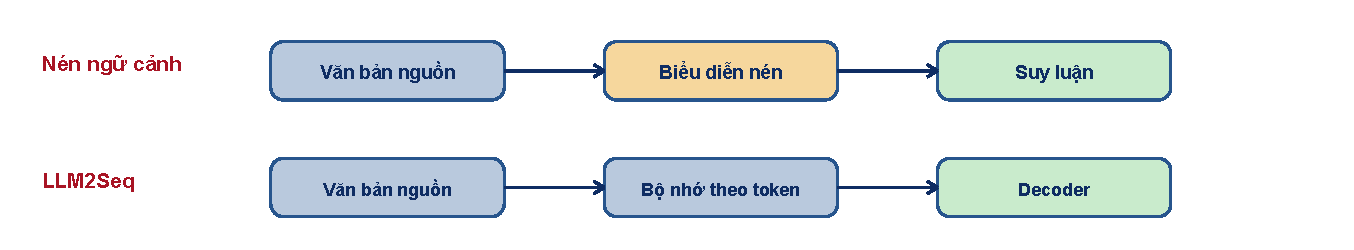
\includegraphics[width=0.96\textwidth,height=0.28\textheight,keepaspectratio]{context_vs_llm2seq_flow.pdf}
  \end{center}
\end{frame}

\begin{frame}{Phát biểu bài toán}
  \begin{block}{Mục tiêu}
    \vspace{0.2em}
    Tìm mô hình ước lượng phân phối của bản tóm tắt $y = (y_1, \ldots, y_n)$ dựa trên văn bản nguồn $x = (x_1, \ldots, x_m)$:
    \vspace{-0.3em}
    $$p(y|x)=\prod_{t=1}^{n}p(y_t \mid y_{<t},x)$$
  \end{block}

  \begin{block}{Công thức hóa LLM2Seq}
    \vspace{0.2em}
    \begin{itemize}
      \item \textbf{Encoder}: Trích xuất hidden states từ LLM, $H=E_{\theta}(x)$.
      \item \textbf{Adapter}: Biến đổi thành không gian bộ nhớ của decoder, $M=A_{\phi}(H)$.
      \item \textbf{Decoder}: Sinh từng token tóm tắt dựa trên token trước đó và bộ nhớ nguồn, $p(y|x)=\prod_{t=1}^{n}p_{\psi}(y_t \mid y_{<t},M)$.
    \end{itemize}
  \end{block}
  \vfill
  \begin{center}
    \small\alert{Việc tách biệt này giúp Encoder tập trung hiểu nguồn, Decoder tập trung sinh văn bản.}
  \end{center}
\end{frame}

\begin{frame}{LLM2Seq: tổng quan kiến trúc}
  \centering
  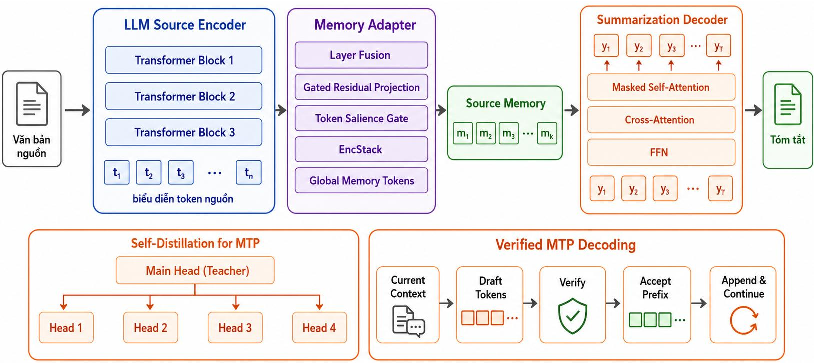
\includegraphics[width=0.98\textwidth,height=0.78\textheight,keepaspectratio]{architecture_crop.pdf}

  \smallnote{Encoder dùng LLM2Vec-Sheared-LLaMA hoặc Qwen3-Embedding-0.6B; decoder nhẹ; MTP có kiểm chứng.}
\end{frame}

\begin{frame}{Adapter: nối biểu diễn nguồn với decoder}
  \begin{columns}[c,onlytextwidth]
    \begin{column}{0.54\textwidth}
      \begin{block}{Các module cốt lõi}
        \begin{enumerate}
          \item \textbf{Token-wise Layer Fusion}: Trộn thông tin từ nhiều layer LLM theo từng token.
          \item \textbf{Gated Residual Projection}: Đưa biểu diễn sang không gian của decoder.
          \item \textbf{Token Salience Gate}: Đánh giá và nhấn mạnh các token mang thông tin quan trọng.
          \item \textbf{EncStack}: Dùng 4 layer Transformer để tinh chỉnh cục bộ bộ nhớ nguồn.
          \item \textbf{Global Memory Tokens}: Cung cấp các token toàn cục cho decoder tham chiếu.
        \end{enumerate}
      \end{block}
    \end{column}
    \begin{column}{0.42\textwidth}
      \begin{center}
      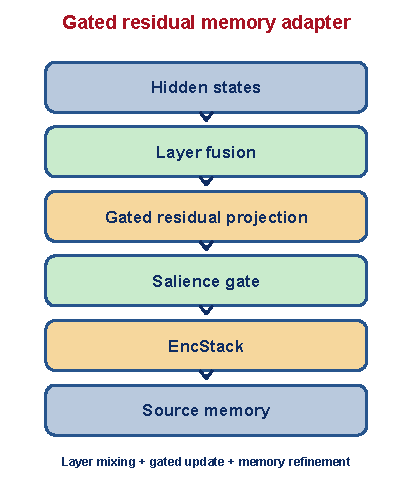
\includegraphics[width=\linewidth,height=0.72\textheight,keepaspectratio]{adapter_flow_redrawn.pdf}
      \end{center}
    \end{column}
  \end{columns}

\end{frame}

\begin{frame}{Huấn luyện theo từng mức can thiệp}
  \vspace{0.2em}
  \begin{center}
    \small\alert{Mỗi giai đoạn chỉ mở thêm phần cần thiết: học đọc nguồn, thích ứng encoder, rồi tăng tốc suy luận.}
  \end{center}

  \vspace{0.25em}
  \begin{columns}[c,onlytextwidth]
    \begin{column}{0.27\textwidth}
      \begin{block}{GĐ 1: Khởi tạo}
        \begin{minipage}[t][3.6cm][t]{\linewidth}
        \small\raggedright
        \textbf{Cố định}\\
        LLM encoder

        \vspace{0.55em}
        \textbf{Cập nhật}\\
        Adapter và decoder

        \vspace{0.55em}
        \textbf{Kết quả}\\
        Decoder học đọc bộ nhớ nguồn $M$.
        \end{minipage}
      \end{block}
    \end{column}
    \begin{column}{0.06\textwidth}
      \centering{\Large$\longrightarrow$}
    \end{column}
    \begin{column}{0.27\textwidth}
      \begin{block}{GĐ 2: Thích ứng}
        \begin{minipage}[t][3.6cm][t]{\linewidth}
        \small\raggedright
        \textbf{Mở khóa}\\
        LoRA trên LLM encoder

        \vspace{0.55em}
        \textbf{Cập nhật}\\
        LoRA, adapter và decoder

        \vspace{0.55em}
        \textbf{Kết quả}\\
        Nguồn khớp hơn với tác vụ tóm tắt.
        \end{minipage}
      \end{block}
    \end{column}
    \begin{column}{0.06\textwidth}
      \centering{\Large$\longrightarrow$}
    \end{column}
    \begin{column}{0.27\textwidth}
      \begin{exampleblock}{GĐ 3: Tăng tốc}
        \begin{minipage}[t][3.6cm][t]{\linewidth}
        \small\raggedright
        \textbf{Cố định}\\
        Mô hình sau GĐ 2

        \vspace{0.55em}
        \textbf{Cập nhật}\\
        4 MTP heads

        \vspace{0.55em}
        \textbf{Kết quả}\\
        Draft-and-verify giảm số bước tự hồi quy.
        \end{minipage}
      \end{exampleblock}
    \end{column}
  \end{columns}
\end{frame}

\begin{frame}{Self-distilled MTP: tăng tốc có kiểm chứng}
  \begin{columns}[T,onlytextwidth]
    \begin{column}{0.48\textwidth}
      \begin{block}{Huấn luyện}
        \begin{minipage}[t][2.1cm][t]{\linewidth}
        \begin{itemize}
          \item Huấn luyện mô hình tóm tắt trước.
          \item Đóng băng encoder, adapter và decoder.
          \item Chỉ cập nhật 4 MTP heads.
        \end{itemize}
        \end{minipage}
      \end{block}
    \end{column}
    \begin{column}{0.48\textwidth}
      \begin{block}{Suy luận}
        \begin{minipage}[t][2.1cm][t]{\linewidth}
        \begin{itemize}
          \item MTP dự đoán vài token tiếp theo.
          \item Decoder kiểm chứng token nháp.
          \item Chỉ ghi token đã được xác nhận.
        \end{itemize}
        \end{minipage}
      \end{block}
    \end{column}
  \end{columns}

  \vfill
  \begin{center}
    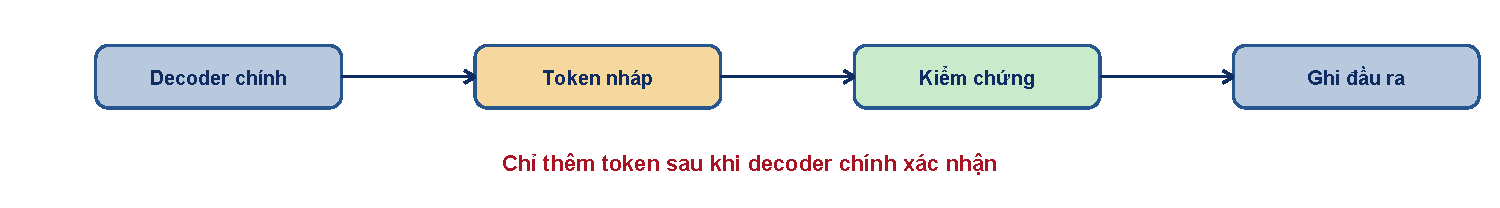
\includegraphics[width=0.88\textwidth,height=0.23\textheight,keepaspectratio]{verified_mtp_flow.pdf}
  \end{center}
\end{frame}

\begin{frame}{Dữ liệu: quy mô train/validation/test}
  \centering
  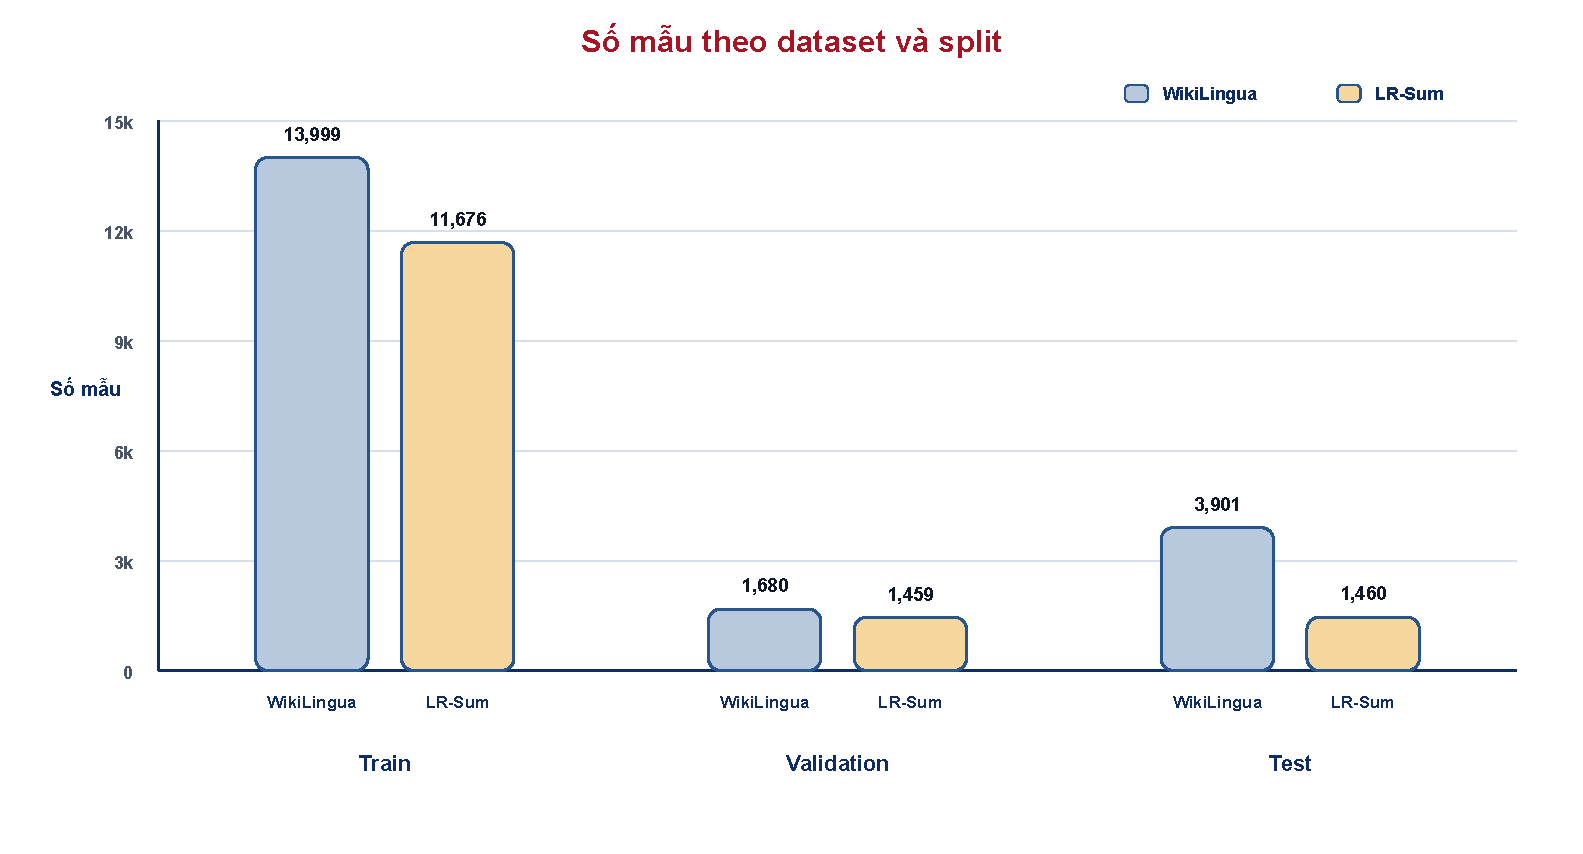
\includegraphics[width=0.96\textwidth,height=0.72\textheight,keepaspectratio]{dataset_split_redrawn.pdf}

  \vfill
  \small\alert{Train dùng để fine-tuning; validation hỗ trợ chọn cấu hình, còn test dùng cho kết quả cuối.}
\end{frame}

\begin{frame}{Dữ liệu: hai nguồn tóm tắt tiếng Việt}
  \centering
  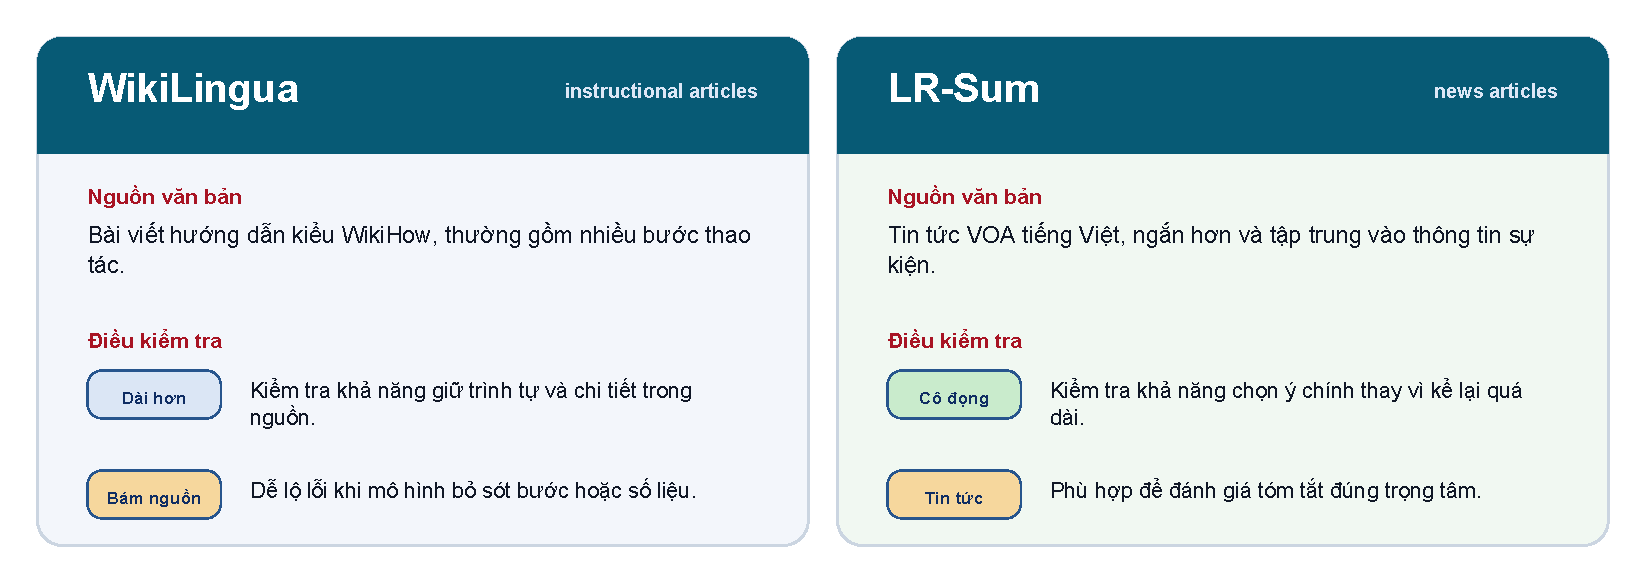
\includegraphics[width=0.98\textwidth,height=0.58\textheight,keepaspectratio]{dataset_sources_cards.pdf}

  \vfill
  \begin{center}
    \small\alert{Hai nguồn dữ liệu tạo áp lực khác nhau: một bên cần giữ trình tự, một bên cần cô đọng ý chính.}
  \end{center}
\end{frame}

\begin{frame}{Thiết lập thí nghiệm}
  \vspace{0.1em}
  \begin{columns}[T,totalwidth=0.98\textwidth]
    \begin{column}{0.545\textwidth}
      \begin{block}{Ba hệ thống so sánh}
        \begin{minipage}[t][4.95cm][t]{\linewidth}
        \small\raggedright
        \renewcommand{\arraystretch}{1.15}
        \begin{tabular}{>{\bfseries}p{0.38\linewidth}>{\raggedright\arraybackslash}p{0.52\linewidth}}
          LLM2Seq-Llama & LLM2Vec-Sheared-LLaMA encoder \\
          LLM2Seq-Qwen & Qwen3-Embedding-0.6B encoder \\
          T5Gemma & T5Gemma-2-1B-1B LoRA baseline \\
        \end{tabular}

        \vspace{0.55em}
        \textbf{Dữ liệu kiểm thử}
        \begin{itemize}
          \setlength{\itemsep}{0.25em}
          \item WikiLingua: tóm tắt hướng dẫn, cần giữ trình tự thao tác.
          \item LR-Sum: văn bản dài, cần cô đọng ý chính.
        \end{itemize}
        \end{minipage}
      \end{block}
    \end{column}
    \hfill
    \begin{column}{0.36\textwidth}
      \begin{exampleblock}{Bốn góc nhìn đánh giá}
        \begin{minipage}[t][4.95cm][t]{\linewidth}
        \small\raggedright
        \begin{itemize}
          \setlength{\itemsep}{0.35em}
          \item \textbf{N-gram}: ROUGE-1/2/L
          \item \textbf{Ngữ nghĩa}: BERTScore mBERT
          \item \textbf{Hành vi sinh}: thống kê độ dài
          \item \textbf{Tốc độ}: token/s và độ trễ
        \end{itemize}
        \vspace{0.25em}
        \centering
        \alert{\small Chất lượng, độ dài và tốc độ được đọc cùng nhau.}
        \end{minipage}
      \end{exampleblock}
    \end{column}
  \end{columns}
\end{frame}

\begin{frame}{Kết quả chính: chất lượng tóm tắt}
  \centering
  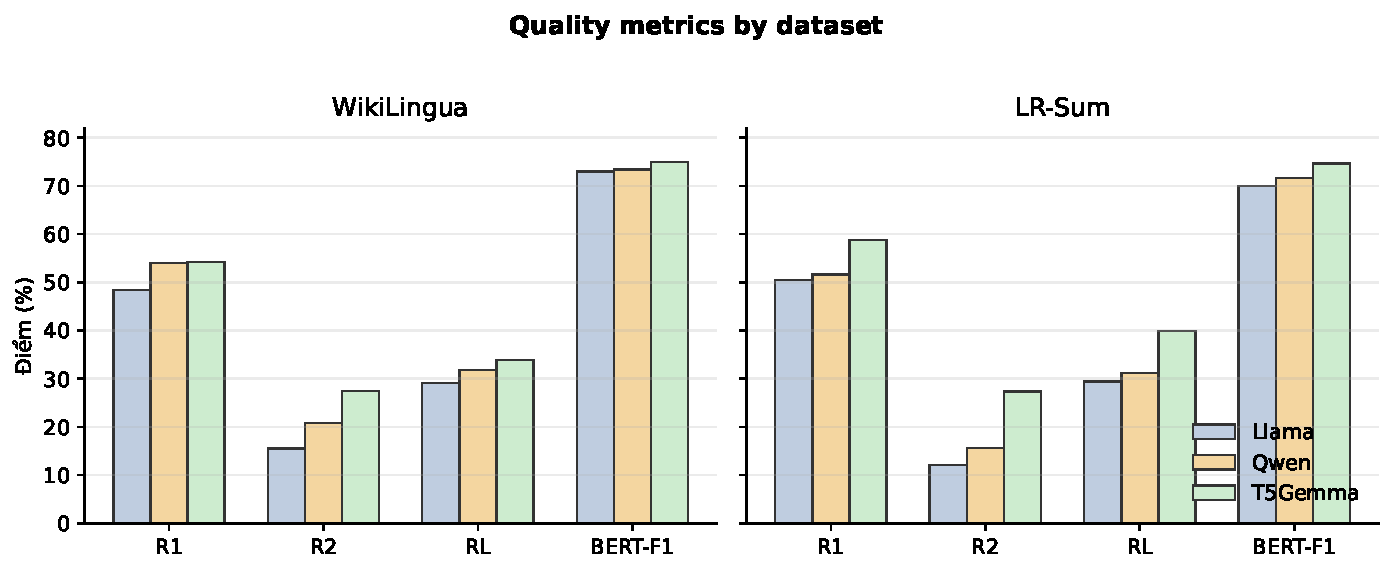
\includegraphics[width=0.98\textwidth,height=0.68\textheight,keepaspectratio]{quality_metrics.pdf}

  \vfill
  \begin{columns}[T,onlytextwidth]
    \begin{column}{0.48\textwidth}
      \small\alert{WikiLingua}: Qwen gần T5Gemma ở ROUGE-1, nhưng thấp hơn ở ROUGE-2 và ROUGE-L.
    \end{column}
    \begin{column}{0.48\textwidth}
      \small\alert{LR-Sum}: Trong cấu hình LLM2Seq, Qwen hơn Llama, nhưng T5Gemma vẫn đạt điểm cao nhất.
    \end{column}
  \end{columns}
\end{frame}

\begin{frame}{Bảng kết quả chính}
  \centering
  \footnotesize
  \setlength{\tabcolsep}{5pt}
  \renewcommand{\arraystretch}{1.12}
  \begin{tabular}{llrrrr}
    \toprule
    Dataset & Model & R-1 & R-2 & R-L & BERT-F1 \\
    \midrule
    \multirow{3}{*}{WikiLingua} & LLM2Seq-Llama & 48.36 & 15.54 & 29.05 & 73.02 \\
    & \cellcolor{LLMBlue!35}LLM2Seq-Qwen & \cellcolor{LLMBlue!35}54.01 & \cellcolor{LLMBlue!35}20.83 & \cellcolor{LLMBlue!35}31.83 & \cellcolor{LLMBlue!35}73.42 \\
    & \cellcolor{LLMGreen!35}T5Gemma & \cellcolor{LLMGreen!35}\textbf{54.24} & \cellcolor{LLMGreen!35}\textbf{27.42} & \cellcolor{LLMGreen!35}\textbf{33.89} & \cellcolor{LLMGreen!35}\textbf{74.98} \\
    \midrule
    \multirow{3}{*}{LR-Sum} & LLM2Seq-Llama & 50.49 & 12.08 & 29.41 & 69.98 \\
    & \cellcolor{LLMBlue!35}LLM2Seq-Qwen & \cellcolor{LLMBlue!35}51.59 & \cellcolor{LLMBlue!35}15.58 & \cellcolor{LLMBlue!35}31.21 & \cellcolor{LLMBlue!35}71.62 \\
    & \cellcolor{LLMGreen!35}T5Gemma & \cellcolor{LLMGreen!35}\textbf{58.79} & \cellcolor{LLMGreen!35}\textbf{27.34} & \cellcolor{LLMGreen!35}\textbf{39.86} & \cellcolor{LLMGreen!35}\textbf{74.65} \\
    \bottomrule
  \end{tabular}

  \vfill
  \begin{columns}[T,onlytextwidth]
    \begin{column}{0.48\textwidth}
      \begin{block}{Nhìn chung}
        \begin{minipage}[t][0.95cm][t]{\linewidth}
        \raggedright Trong cấu hình LLM2Seq, Qwen tốt hơn Llama trên cả hai bộ dữ liệu.
        \end{minipage}
      \end{block}
    \end{column}
    \begin{column}{0.48\textwidth}
      \begin{block}{So với T5Gemma}
        \begin{minipage}[t][0.95cm][t]{\linewidth}
        \raggedright T5Gemma vẫn mạnh hơn, nhất là ROUGE-2 và ROUGE-L.
        \end{minipage}
      \end{block}
    \end{column}
  \end{columns}

\end{frame}

\begin{frame}{Kết quả độ dài: không chỉ nhìn ROUGE}
  \centering
  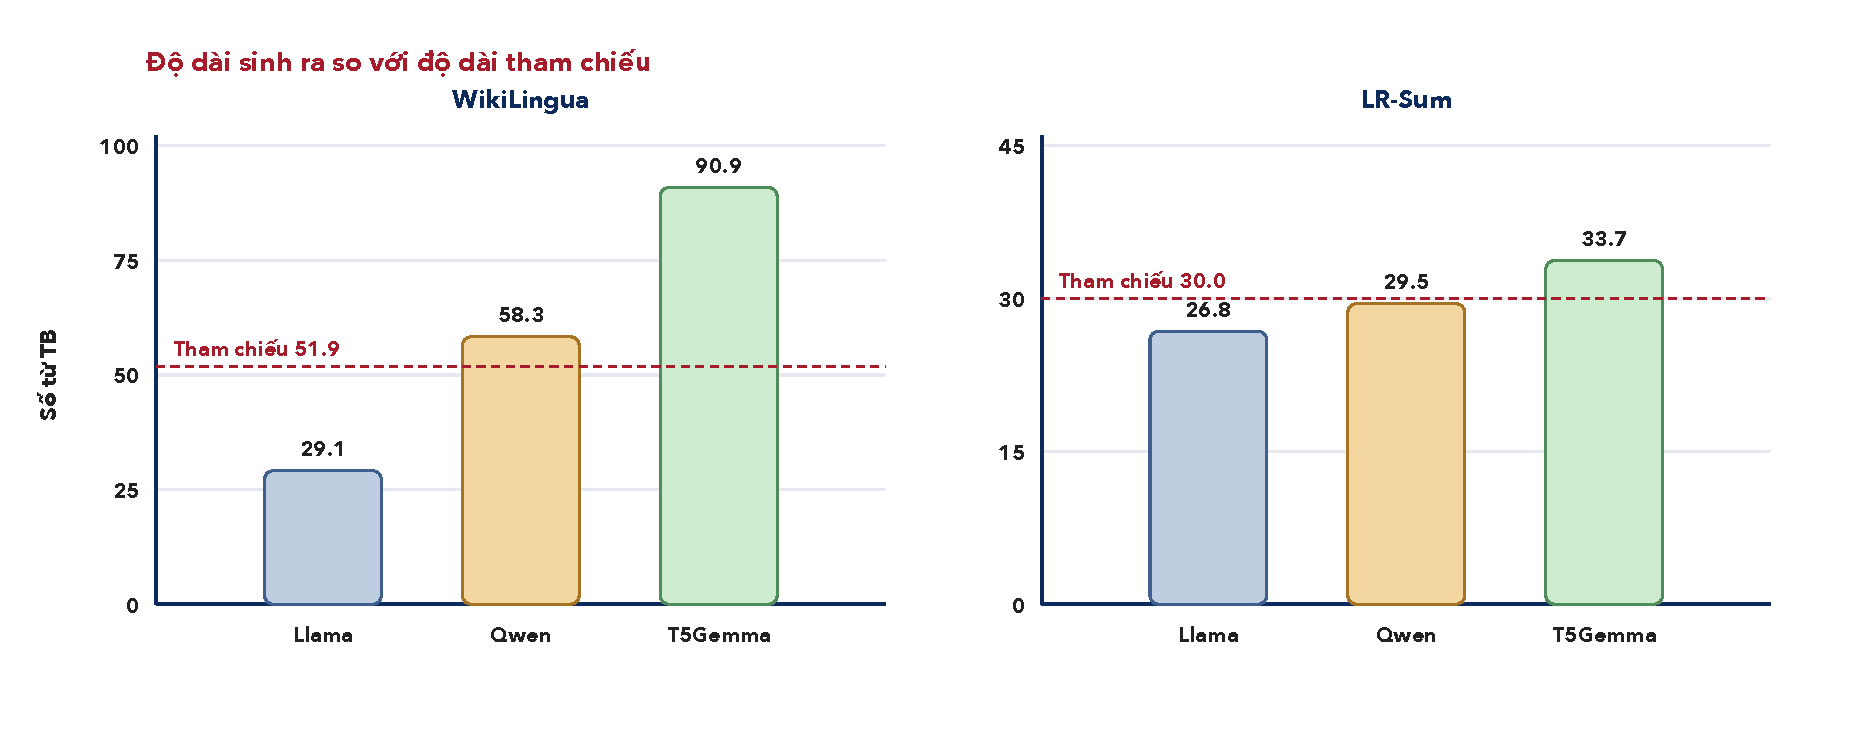
\includegraphics[width=0.90\textwidth,height=0.67\textheight,keepaspectratio]{length_behavior.pdf}

  \vfill
  \small\alert{Nhận xét}: Llama thường sinh ngắn. Qwen gần độ dài tham chiếu hơn. T5Gemma dài hơn, tăng độ trùng nhưng kém cô đọng hơn.
\end{frame}

\begin{frame}{Ví dụ định tính: Qwen giữ ý nguồn tốt hơn}
  \begin{block}{Văn bản nguồn (WikiLingua)}
    \small \textit{... Tùy vào loại da và mức độ nghiêm trọng của mụn ẩn mà bạn nên cân nhắc giữa phương pháp chườm ấm với chườm lạnh. Chườm ấm giúp làm khô mụn ẩn; chườm lạnh giúp giảm sưng đau. Không nên chườm đá trong giai đoạn đầu. Nếu là mụn lớn, viêm nghiêm trọng, nên chườm ấm để rút dịch ...}
  \end{block}

  \vspace{0.05em}
  \begin{columns}[T,onlytextwidth]
    \begin{column}{0.305\textwidth}
      \begin{alertblock}{LLM2Seq-Llama}
        \begin{minipage}[t][3.05cm][t]{\linewidth}
        \scriptsize\raggedright
        \textbf{Sinh ra}\\
        Dùng gel lô hội.\\
        Thoa sữa rửa mặt nhẹ dịu.\\
        Dù bằng dầu tràm trà.\\
        Dưỡng ẩm cho da.

        \vspace{0.35em}
        \textbf{Hành vi}\\
        Quá ngắn, bỏ mất ý chính và tự thêm chi tiết ngoài nguồn.
        \end{minipage}
      \end{alertblock}
    \end{column}
    \hfill
    \begin{column}{0.305\textwidth}
      \begin{exampleblock}{LLM2Seq-Qwen}
        \begin{minipage}[t][3.05cm][t]{\linewidth}
        \scriptsize\raggedright
        \textbf{Sinh ra}\\
        Chườm đá viên lên mụn.\\
        Chườm gạc ấm lên mụn để giảm đau.\\
        Sử dụng tinh dầu tràm trà...

        \vspace{0.35em}
        \textbf{Hành vi}\\
        Bắt được ý chính về chườm ấm/lạnh, nhưng còn lẫn chỉ dẫn.
        \end{minipage}
      \end{exampleblock}
    \end{column}
    \hfill
    \begin{column}{0.305\textwidth}
      \begin{block}{T5Gemma}
        \begin{minipage}[t][3.05cm][t]{\linewidth}
        \scriptsize\raggedright
        \textbf{Sinh ra}\\
        Chườm ấm hoặc chườm lạnh.\\
        Thử dùng táo và mật ong...\\
        Dùng tinh dầu tràm trà...

        \vspace{0.35em}
        \textbf{Hành vi}\\
        Diễn đạt tự nhiên hơn, nhưng sinh thêm thông tin phụ.
        \end{minipage}
      \end{block}
    \end{column}
  \end{columns}
\end{frame}

\begin{frame}{MTP trên WikiLingua: tăng tốc vừa phải}
  \centering
  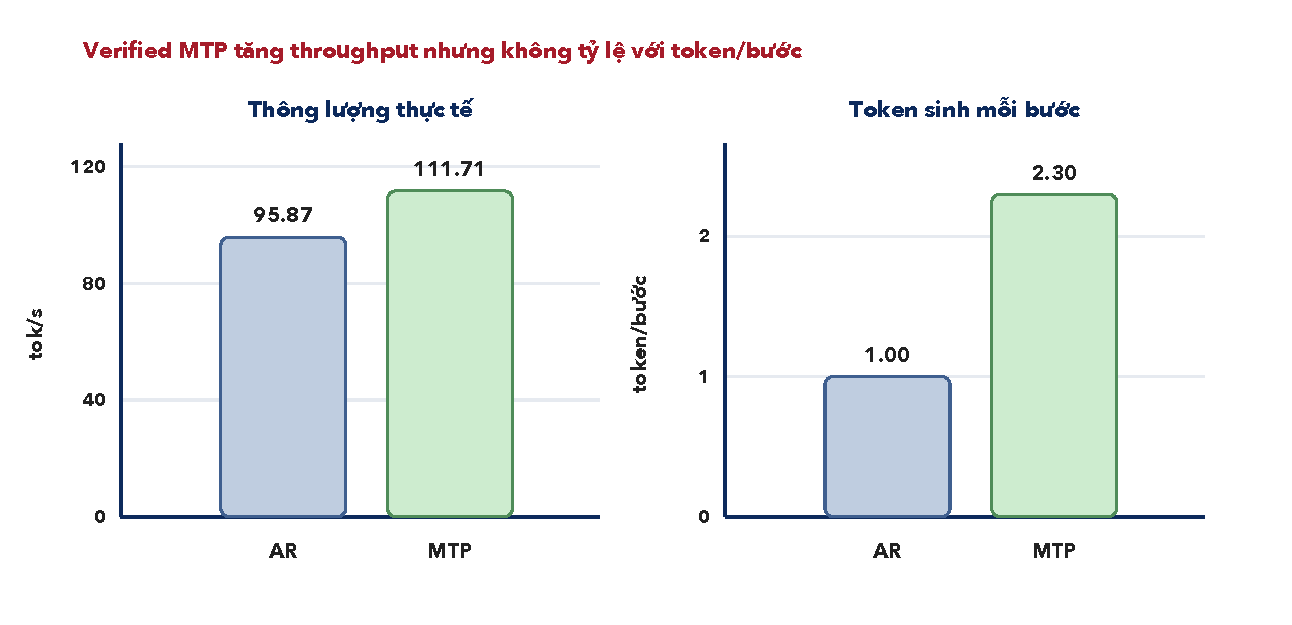
\includegraphics[width=0.98\textwidth,height=0.62\textheight,keepaspectratio]{mtp_speed.pdf}

  \vfill
  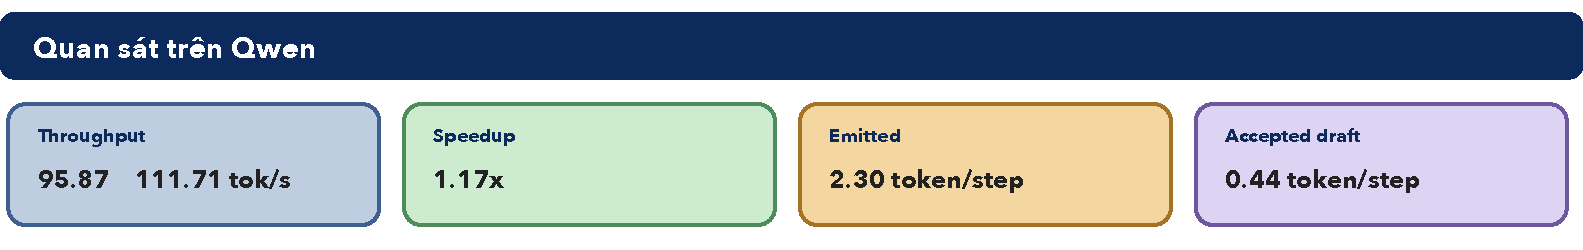
\includegraphics[width=0.98\textwidth,height=0.23\textheight,keepaspectratio]{qwen_mtp_observation.pdf}
\end{frame}

\begin{frame}{Vì sao MTP trên WikiLingua chưa tăng tốc mạnh?}
  \centering
  
\includegraphics[width=0.98\textwidth,height=0.56\textheight,keepaspectratio]{mtp_latency_accounting.pdf}

  \vspace{0.2em}
  \begin{columns}[T,onlytextwidth]
    \begin{column}{0.48\textwidth}
      \small
      \begin{block}{Nếu tính lý tưởng}
        \begin{minipage}[t][0.72cm][t]{\linewidth}
        \raggedright 2.30 token/bước tương ứng 0.339s lý tưởng; đo thực tế 0.662s.
        \end{minipage}
      \end{block}
    \end{column}
    \begin{column}{0.48\textwidth}
      \small
      \begin{block}{Phần còn lại}
        \begin{minipage}[t][0.72cm][t]{\linewidth}
        \raggedright Chênh 0.323s chủ yếu đến từ bước kiểm chứng, cache và chi phí Python.
        \end{minipage}
      \end{block}
    \end{column}
  \end{columns}
\end{frame}

\begin{frame}{Demo hệ thống}
  \begin{columns}[T,onlytextwidth]
    \begin{column}{0.49\textwidth}
      \centering
      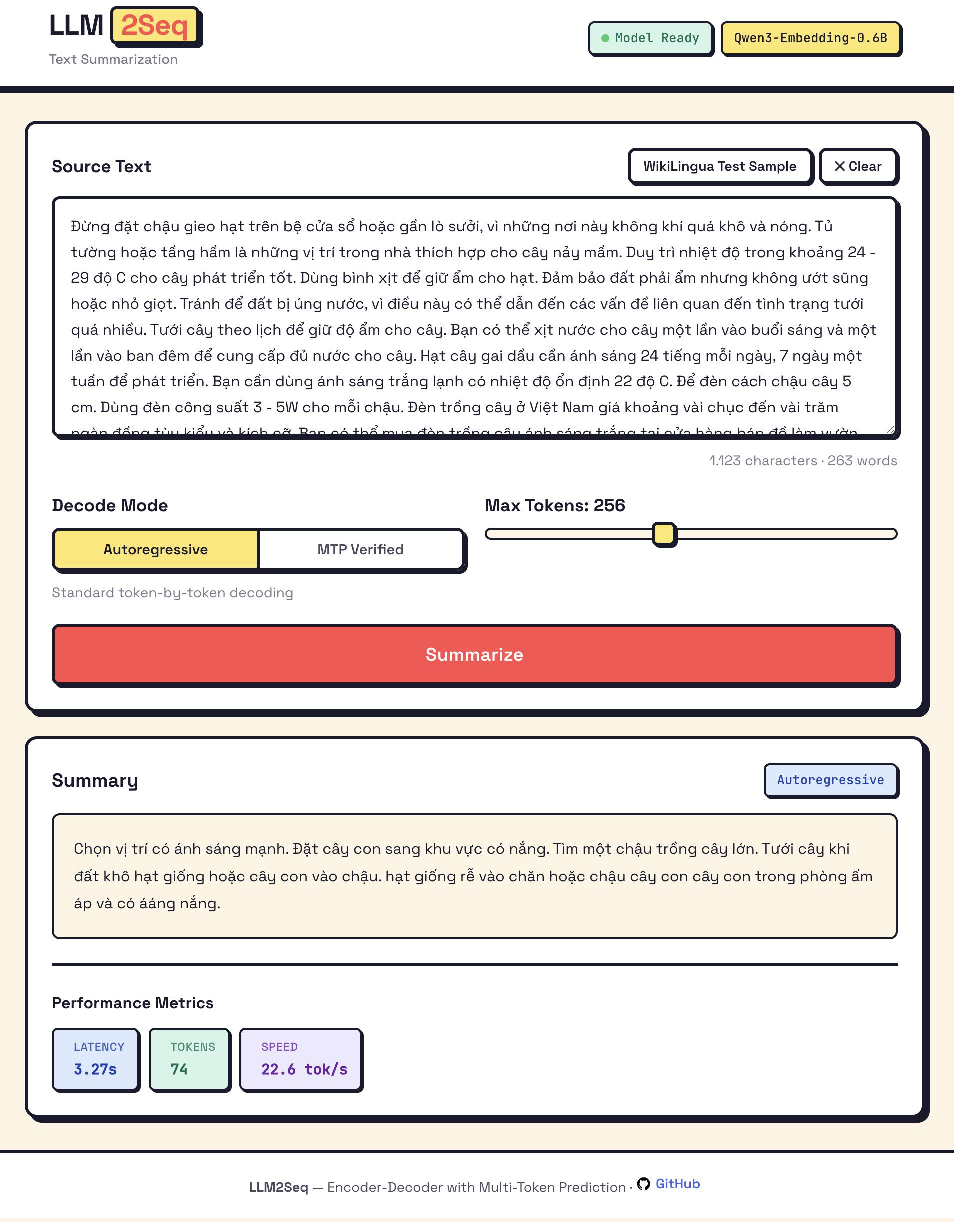
\includegraphics[width=\linewidth,height=0.73\textheight,keepaspectratio]{demo_autoregressive_cropped.pdf}

      \scriptsize Autoregressive
    \end{column}
    \begin{column}{0.49\textwidth}
      \centering
      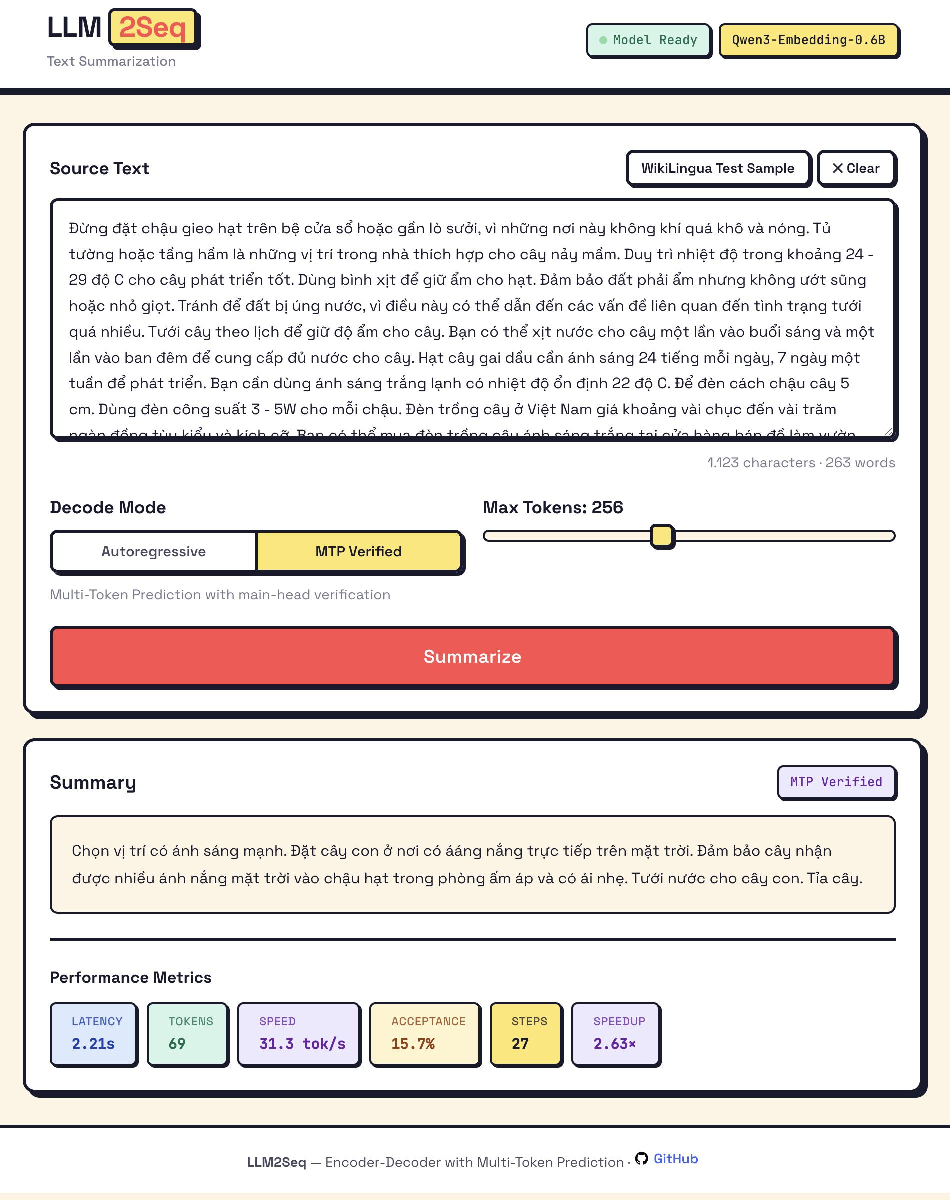
\includegraphics[width=\linewidth,height=0.73\textheight,keepaspectratio]{demo_mtp_cropped.pdf}

      \scriptsize Verified MTP
    \end{column}
  \end{columns}
\end{frame}

\begin{frame}{Thảo luận và hạn chế}
  \begin{columns}[T,onlytextwidth]
    \begin{column}{0.48\textwidth}
      \begin{block}{Kết quả rút ra}
        \begin{minipage}[t][3.35cm][t]{\linewidth}
        \begin{itemize}
          \item Có thể dùng LLM làm bộ đọc nguồn cho decoder.
          \item Trong cấu hình LLM2Seq, Qwen tốt hơn Llama trên cả hai bộ dữ liệu.
          \item Verified MTP giúp chạy nhanh hơn trên WikiLingua.
        \end{itemize}
        \end{minipage}
      \end{block}
    \end{column}
    \begin{column}{0.48\textwidth}
      \begin{block}{Hạn chế hiện tại}
        \begin{minipage}[t][3.35cm][t]{\linewidth}
        \begin{itemize}
          \item Chưa chạy đầy đủ ablation cho từng phần của adapter.
          \item Chưa có đánh giá thủ công về factuality / độ đúng nội dung.
          \item MTP vẫn tốn chi phí kiểm chứng và cache.
        \end{itemize}
        \end{minipage}
      \end{block}
    \end{column}
  \end{columns}

  \vfill
  \begin{center}
    \normalsize\alert{Trong cấu hình LLM2Seq, Qwen tốt hơn Llama, nhưng chưa vượt T5Gemma.}
  \end{center}
\end{frame}

\begin{frame}{Thông điệp chính}
  \vspace{0.3em}
  \begin{itemize}
    \item LLM2Seq chuyển hidden states từ LLM encoder thành source memory cho decoder.
    \item Trong cấu hình LLM2Seq, Qwen tốt hơn Llama trên WikiLingua và LR-Sum.
    \item T5Gemma vẫn mạnh hơn, đặc biệt ở ROUGE-2 và ROUGE-L.
    \item Verified MTP đạt 1.17x trên WikiLingua, nhưng còn tốn chi phí kiểm chứng.
  \end{itemize}

  \vfill
  \begin{block}{Bước tiếp theo}
    Chạy thêm ablation cho adapter, đánh giá factuality / độ đúng nội dung, và tối ưu verified decoding.
  \end{block}
\end{frame}

\begin{frame}{Hỏi đáp}
  \centering
  \vspace{1.0em}
  {\Huge\bfseries Thank you}

  \vspace{0.45em}
  {\Large Q\&A}

  \begin{tikzpicture}[remember picture,overlay]
    \node[anchor=south east,align=right,xshift=-1.98cm,yshift=0.85cm] at (current page.south east) {
      \scriptsize GitHub:\\[-0.1em]
      \scriptsize\href{https://github.com/BienKieu1411/LLM2Seq}{github.com/BienKieu1411/LLM2Seq}
    };
    \node[anchor=south east,xshift=-0.45cm,yshift=0.54cm] at (current page.south east) {
      \href{https://github.com/BienKieu1411/LLM2Seq}{
\includegraphics[width=1.25cm]{github_qr.pdf}}
    };
  \end{tikzpicture}
\end{frame}

\end{document}
